\newcommand{\cccnormspacing}{\baselineskip=12pt}
\newcommand{\cccnormspacingcenter}{\centering\arraybackslash\cccnormspacing}


\section{Penentuan Kebutuhan Pengguna}

Setelah mengidentifikasi konteks penggunaan dari aplikasi Digital Wellbeing, maka taha selanjutnya adalah menentukan kebutuhan pengguna. Pada tahap ini akan dilakukan analisis terhadap skenario pengguna, analisis tipe interaksi dari desain, analisis fitur-fitur yang dibutuhkan, analisis prinsip desain, serta analisis usability dan user experience goals yang dibutuhkan pengguna. Kebutuhan-kebutuhan ini digunakan untuk membangun prototipe aplikasi solusi.

\subsection{Skenario Pengguna}
Sebelum menentukan solusi desain yang perlu memenuhi kebutuhan pengguna, skenario pengguna disusun berdasarkan persona yang dipilih, yaitu persona Maya. Skenario pengguna mengembangkan persona lebih lanjut dengan memberikan gambaran tentang bagaimana persona tersebut menggunakan aplikasi untuk mencapai tujuan-tujuannya. Penulisan skenario dalam bentuk narasi adalah alat bantu desain yang efektif untuk mengkomunikasikan ide dari desain tersebut, dalam membantu penggunanya. \parencite{cooper2014face} Berikut adalah skenario-skenario pengguna dari persona Maya yang mendeskripsikan contoh kasus penggunaan solusi desain untuk aplikasi Digital Wellbeing
\begin{enumerate}
  \item Maya sedang bekerja menggunakan laptopnya, saat ia sedang merasa sedikit bosan dan tiba-tiba mendapat perasaan untuk memeriksa media sosial lewat smartphonenya. Tanpa sadar, Maya sudah bermain media sosial selama setengah jam ketika rekannya bertanya tentang pekerjaannya. Bagaimana aplikasi Digital Wellbeing dapat membantu Maya dalam fokus dalam aktivitasnya di jam kerja?
  \item Maya ingin menganalisis penggunaan \textit{smartphone} dengan melihat seberapa sering ia menggunakan aplikasi favoritnya. Lalu Maya menemukan bahwa ia menggunakan Instagram dan Twitter terlalu sering setiap harinya. Maya ingin memasang batas waktu penggunaan agar pelan-pelan bisa dikurangi. Bagaimana aplikasi Digital Wellbeing dapat memberikan sugesti  tentang penggunaan \textit{smartphone} yang wajar dan batas apa saja yang Maya bisa pasang untuk membantu memperbaiki kebiasaannya?
  \item Maya sedang memulai minggu kerjanya di hari senin, dan ia ingat untuk mengatur jadwal pembatasan akses dan notifikasi dari aplikasi. Bagaimana cara Maya bisa mengatur jadwalnya agar bisa sesuai dengan jam kerjanya yang bervariasi?
  \item Mendekati akhir hari kerjanya, Maya menyelesaikan tugasnya lebih cepat dari biasanya dan ingin bermain di smartphonenya. Namun ia telah memasang restriksi sebelumnya yang akan diangkat setelah jam kerjanya selesai. Bagaimana aplikasi Digital Wellbeing dapat memberikan leluasa kepada Maya tanpa menghapus pengaturan yang telah dipasang?
  \item Maya ingin beristirahat untuk mengakhiri harinya. Namun Maya lupa waktu ketika sedang bermain dengan smartphonenya sehingga ia melewati jam tidurnya selama satu jam. Maya ingin memasang pengingat pada \textit{smartphone} untuk menepati jam tidurnya agar setiap pagi ia bisa bangun denga tepat waktu dengan segar. Bagaimana aplikasi Digital Wellbeing dapat membantu mencapai tujuannya?
\end{enumerate}

\subsection{Analisis Tipe Interaksi}

Sebelum menentukan elemen-elemen dari desain, perlu ditentukan tipe interaksi yang akan menjadi konsep dari prototipe aplikasi solusi. Tipe interaksi yang dibahas akan mengacu pada studi literatur bagian \ref{subsec:tipe_interaksi}. Menurut observasi pada aplikasi Digital Wellbeing awal, dapat ditentukan bahwa tipe interaksi yang diterapkan adalah \textit{instructing} dengan melihat bagaimana aplikasi membantu penggunanya menyetel pengaturan-pengaturan. Sesuai dengan kebutuhan pengguna yang dianalisis, terutama kebutuhan KP-01 tentang efisiensi dalam pengaturan aplikasi, tipe interaksi ini akan dipertahankan melihat kekuatan tipe interaksi dalam menyediakan kecepatan dan efisiensi dalam berinteraksi.

Dari menganalisis kebutuhan pengguna, ditemukan bahwa diperlukan tipe interaksi tambahan. Menurut kebutuhan KP-03, pengguna membutuhkan sebuah fitur rekomendasi untuk memberikan informasi tentang kebiasaan digital yang baik. Selain itu, kebutuhan KP-09 menyebutkan bahwa pengguna membutuhkan interaksi yang terasa lebih personal dengan aplikasi. Hal-hal tersebut menunjukkan bahwa solusi desain memerlukan tipe interaksi \textit{responding}, di mana sistem akan menginisiasi interaksi kepada pengguna dan menunggu balasan. Tipe interaksi ini akan difokuskan pada sistem rekomendasi kebiasaan digital yang sehat untuk pengguna, serta pada pesan-pesan pengingat sesuai dengan fitur yang memanfaatkannya. Walaupun interaksi ini diinisiasi oleh sistem, pengguna tetap dapat mengaturnya sesuai dengan kebutuhan, dan penerapannya akan dianalisis lebih lanjut pada tahap evaluasi.

Tipe interaksi lain tidak akan dipertimbangkan ke dalam solusi desain. Tipe interaksi \textit{conversing} dinilai akan membuat pengguna kurang efisien dalam melakukan pengaturan. Sedangkan tipe interaksi \textit{manipulating} dan \textit{exploring} dinilai tidak relevan melihat tidak adanya kebutuhan pengguna terhadap objek-objek yang lebih nyata atau lingkungan sistem yang dapat dieksplorasi.

\subsection{Analisis Fitur}

Dari menganalisis kebutuhan dan tujuan pengguna, maka dapat ditentukan fitur-fitur yang diperlukan dari aplikasi solusi desain. Sebagian besar fitur dari aplikasi awal Digital Wellbeing akan dipertahankan dalam perancangan solusi, namun akan dilakukan modifikasi sesuai dengan kebutuhan pengguna. Pada Tabel \ref{tab:daftar_fitur} dapat ditemukan fitur-fitur yang akan diimplementasi. Status Fitur menunjukkan fitur yang sudah diimplementasi sebelumnya, fitur yang akan dimodifikasi, atau fitur yang baru diimplementasi.
% $ Kalau perlu fungsionalitas 
% Keterkaitan Fungsionalitas mendahulukan fungsionalitas dari aplikasi Digital Wellbeing melihat terdapat beberapa fungsionalitas umum yang telah terdapat di aplikasi.

% $ Kalau perlu fungsionalitas
% \RaggedLeft
% \begin{small}
% \begin{longtable}[c]{|W{c}{0.06\textwidth}|>{\cccnormspacingcenter}m{0.15\textwidth}|>{\cccnormspacing}m{0.3\textwidth}|>{\cccnormspacingcenter}m{0.12\textwidth}|>{\cccnormspacingcenter}m{0.16\textwidth}|>{\cccnormspacingcenter}m{0.18\textwidth}|}
%   \caption{Daftar Fitur Prototipe Aplikasi}
%   \label{tab:daftar_fitur} \\
%   \hline \rowcolor[HTML]{A3E5F5}
%   \textbf{ID} & \textbf{Fitur} & \centering\textbf{Penjelasan} & \textbf{Tipe Fitur} & \textbf{Keterkaitan Kebutuhan \& Tujuan} & \textbf{Keterkaitan Fungsionalitas} \\ \hline \endfirsthead
%   \hline \rowcolor[HTML]{A3E5F5}
%   \textbf{ID} & \textbf{Fitur} & \centering\textbf{Penjelasan} & \textbf{Tipe Fitur} & \textbf{Keterkaitan Kebutuhan \& Tujuan} & \textbf{Keterkaitan Fungsionalitas} \\ \hline \endhead
%   \hline \endfoot

%   F-01 & \textit{Usage tracker} & Melacak penggunaan \textit{smartphone} dan aplikasi-aplikasi dari sisi lama penggunaan, jumlah pembukaan, dan notifikasi yang diterima & Sudah ada & KP-04, UG-04 & FD-01, FD-02 \\ \hline
%   F-02 & \textit{Pie chart} & Menampilkan laporan data penggunaan \textit{smartphone} dan aplikasi-aplikasi untuk hari yang sedang berlangsung & Sudah ada & KP-04, UG-04 & FD-03 \\ \hline
%   F-03 & \textit{Bar chart} & Menampilkan ringkasan laporan data penggunaan \textit{smartphone} dan aplikasi-aplikasi & Modifikasi & KP-04, UG-04 & FD-03 \\ \hline
%   F-04 & \textit{Date range selector} & Memilih rentang tanggal untuk tampilan laporan penggunaan & Baru & KP-04, UG-04 & FU-03 \\ \hline
%   F-05 & \textit{Usage Summary} & Menampilkan ringkasan singkat tentang laporan penggunaan \textit{smartphone} dan aplikasi & Baru & KP-04, UG-04 & FU-03 \\ \hline
%   F-06 & Rekomendasi perbaikan perilaku & Memberikan rekomendasi berdasarkan perilaku dari pengguna tentang aksi yang dapat dilakukan untuk memperbaiki kebiasaan digital pengguna & Baru & KP-03, UG-04 & - \\ \hline
%   F-07 & \textit{Dashboard Widget} & Menampilkan laporan penggunaan \textit{smartphone} dan aplikasi untuk hari yang sedang berlangsung & Modifikasi & KP-02, UG-04 & FD-03, FD-04 \\ \hline
%   F-08 & \textit{App Timer} & Membatasi waktu penggunaan aplikasi harian & Sudah ada & UG-03 & FD-05 \\ \hline
%   F-09 & \textit{App Timer Widget}  & Menampilkan daftar sisa waktu penggunaan aplikasi yang dipasang App Timer & Baru & KP-02, UG-03 & FU-06 \\ \hline
%   F-10 & Daftar aplikasi & Menampilkan seluruh aplikasi yang terdapat di \textit{smartphone} untuk diberikan aksi lanjutan sesuai konteks fitur & Sudah ada & KP-01 & FD-04 \\ \hline
%   F-11 & \textit{Search bar} & Mencari aplikasi yang terdapat pada daftar & Baru & KP-01 & - \\ \hline
%   F-12 & \textit{App Grouping} & Mengelompokkan aplikasi-aplikasi berdasarkan kategori yang ditentukan pengguna & Baru & KP-01 & - \\ \hline
%   F-13 & \textit{Focus Mode} & Memblokir akses aplikasi dan informasi yang diberikan oleh aplikasi  pilihan untuk waktu yang ditentukan atau sehari penuh & Modifikasi & UG-02, UG-03 & FD-08, FD-09 \\ \hline
%   F-14 & \textit{Take a break} & Menunda pemblokiran dari fitur-fitur untuk waktu yang ditentukan & Modifikasi & KP-08, UG-07 & FD-11 \\ \hline
%   F-15 & \textit{Turn off for now} & Mematikan pemblokiran dari fitur-fitur untuk sehari penuh & Modifikasi & KP-08, UG-07 & FD-11 \\ \hline
%   F-16 & \textit{Focus Mode Widget} & Menampilkan jadwal aktivasi Focus Mode dan fungsionalitas aktivasi dari fitur Focus Mode & Baru & KP-02, UG-02 & FU-06 \\ \hline
%   F-17 & \textit{Bedtime Mode} & Mengubah \textit{smartphone} ke dalam perilaku mode tidur pada jadwal yang ditentukan & Modifikasi & UG-06 & FD-12 \\ \hline
%   F-18 & \textit{Greyscale screen} & Mengubah warna layar \textit{smartphone} menjadi hitam-putih & Sudah ada & UG-02 & FD-15 \\ \hline
%   F-19 & \textit{Do Not Disturb} & Mengalihkan pengguna ke layar pengaturan Do Not Disturb bawaan \textit{smartphone} & Sudah ada & UG-02 & - \\ \hline
%   F-20 & Pengaturan notifikasi & Mengalihkan pengguna ke layar pengaturan notifikasi aplikasi bawaan \textit{smartphone} & Sudah ada & UG-02 & - \\ \hline
%   F-21 & Daftar Jadwal Aktivasi & Memberikan pengguna kemampuan untuk mengatur 0 atau lebih jadwal aktivasi fitur & Modifikasi & KP-07 & FD-10 \\ \hline
%   F-22 & \textit{Goal Reminder} & Menambah pesan pengingat opsional yang akan ditambahkan pada pesan yang diberikan oleh fitur tertentu & Baru & KP-09, UG-05 & FU-13 \\ \hline
%   F-23 & \textit{Daily Summary Notification} & Memberikan notifikasi berisi ringkasan penggunaan \textit{smartphone} harian dan pembanding dengan data hari kemarin & Baru & KP-03, KP-11, UG-04 & FU-07 \\ \hline
%   F-24 & \textit{Strictness level} & Memilih tingkat keketatan dengan mengatur kemampuan fitur-fitur tertentu & Baru & KP-05, UG-01 & - \\ \hline
%   F-25 & \textit{Settings lock} & Mengunci pengaturan fitur-fitur tertentu dari pengubahan untuk waktu yang ditentukan & Baru & KP-06, UG-01 & - \\ \hline

% \end{longtable}
% \end{small}
% \justifying
% \FloatBarrier

% $ Kalau perlu fungsionalitas dan landscape
% \newpage
% \begin{landscape}
%   \RaggedLeft
%   \begin{small}
% \begin{longtable}[c]{|W{c}{0.06\textwidth}|>{\cccnormspacingcenter}m{0.15\textwidth}|>{\cccnormspacing}m{0.9\textwidth}|>{\cccnormspacingcenter}m{0.12\textwidth}|>{\cccnormspacingcenter}m{0.18\textwidth}|>{\cccnormspacingcenter}m{0.18\textwidth}|}
%   \caption{Daftar Fitur Prototipe Aplikasi}
%   \label{tab:daftar_fitur} \\
%   \hline \rowcolor[HTML]{A3E5F5}
%   \textbf{ID} & \textbf{Fitur} & \centering\textbf{Penjelasan} & \textbf{Tipe Fitur} & \textbf{Keterkaitan Kebutuhan \& Tujuan} & \textbf{Keterkaitan Fungsionalitas} \\ \hline \endfirsthead
%   \hline \rowcolor[HTML]{A3E5F5}
%   \textbf{ID} & \textbf{Fitur} & \centering\textbf{Penjelasan} & \textbf{Tipe Fitur} & \textbf{Keterkaitan Kebutuhan \& Tujuan} & \textbf{Keterkaitan Fungsionalitas} \\ \hline \endhead
%   \hline \endfoot

%   F-01 & \textit{Usage tracker} & Melacak penggunaan \textit{smartphone} dan aplikasi-aplikasi dari sisi lama penggunaan, jumlah pembukaan, dan notifikasi yang diterima & Sudah ada & KP-04, UG-04 & FD-01, FD-02 \\ \hline
%   F-02 & \textit{Pie chart} & Menampilkan laporan data penggunaan \textit{smartphone} dan aplikasi-aplikasi untuk hari yang sedang berlangsung & Sudah ada & KP-04, UG-04 & FD-03 \\ \hline
%   F-03 & \textit{Bar chart} & Menampilkan ringkasan laporan data penggunaan \textit{smartphone} dan aplikasi-aplikasi & Modifikasi & KP-04, UG-04 & FD-03 \\ \hline
%   F-04 & \textit{Date range selector} & Memilih rentang tanggal untuk tampilan laporan penggunaan & Baru & KP-04, UG-04 & FU-03 \\ \hline
%   F-05 & \textit{Usage Summary} & Menampilkan ringkasan singkat tentang laporan penggunaan \textit{smartphone} dan aplikasi & Baru & KP-04, UG-04 & FU-03 \\ \hline
%   F-06 & Rekomendasi perbaikan perilaku & Memberikan rekomendasi berdasarkan perilaku dari pengguna tentang aksi yang dapat dilakukan untuk memperbaiki kebiasaan digital pengguna & Baru & KP-03, UG-04 & - \\ \hline
%   F-07 & \textit{Dashboard Widget} & Menampilkan laporan penggunaan \textit{smartphone} dan aplikasi untuk hari yang sedang berlangsung & Modifikasi & KP-02, UG-04 & FD-03, FD-04 \\ \hline
%   F-08 & \textit{App Timer} & Membatasi waktu penggunaan aplikasi harian & Sudah ada & UG-03 & FD-05 \\ \hline
%   F-09 & \textit{App Timer Widget}  & Menampilkan daftar sisa waktu penggunaan aplikasi yang dipasang App Timer & Baru & KP-02, UG-03 & FU-06 \\ \hline
%   F-10 & Daftar aplikasi & Menampilkan seluruh aplikasi yang terdapat di \textit{smartphone} untuk diberikan aksi lanjutan sesuai konteks fitur & Sudah ada & KP-01 & FD-04 \\ \hline
%   F-11 & \textit{Search bar} & Mencari aplikasi yang terdapat pada daftar & Baru & KP-01 & - \\ \hline
%   F-12 & \textit{App Grouping} & Mengelompokkan aplikasi-aplikasi berdasarkan kategori yang ditentukan pengguna & Baru & KP-01 & - \\ \hline
%   F-13 & \textit{Focus Mode} & Memblokir akses aplikasi dan informasi yang diberikan oleh aplikasi  pilihan untuk waktu yang ditentukan atau sehari penuh & Modifikasi & UG-02, UG-03 & FD-08, FD-09 \\ \hline
%   F-14 & \textit{Take a break} & Menunda pemblokiran dari fitur-fitur untuk waktu yang ditentukan & Modifikasi & KP-08, UG-07 & FD-11 \\ \hline
%   F-15 & \textit{Turn off for now} & Mematikan pemblokiran dari fitur-fitur untuk sehari penuh & Modifikasi & KP-08, UG-07 & FD-11 \\ \hline
%   F-16 & \textit{Focus Mode Widget} & Menampilkan jadwal aktivasi Focus Mode dan fungsionalitas aktivasi dari fitur Focus Mode & Baru & KP-02, UG-02 & FU-06 \\ \hline
%   F-17 & \textit{Bedtime Mode} & Mengubah \textit{smartphone} ke dalam perilaku mode tidur pada jadwal yang ditentukan & Modifikasi & UG-06 & FD-12 \\ \hline
%   F-18 & \textit{Greyscale screen} & Mengubah warna layar \textit{smartphone} menjadi hitam-putih & Sudah ada & UG-02 & FD-15 \\ \hline
%   F-19 & \textit{Do Not Disturb} & Mengalihkan pengguna ke layar pengaturan Do Not Disturb bawaan \textit{smartphone} & Sudah ada & UG-02 & - \\ \hline
%   F-20 & Pengaturan notifikasi & Mengalihkan pengguna ke layar pengaturan notifikasi aplikasi bawaan \textit{smartphone} & Sudah ada & UG-02 & - \\ \hline
%   F-21 & Daftar Jadwal Aktivasi & Memberikan pengguna kemampuan untuk mengatur 0 atau lebih jadwal aktivasi fitur & Modifikasi & KP-07 & FD-10 \\ \hline
%   F-22 & \textit{Goal Reminder} & Menambah pesan pengingat opsional yang akan ditambahkan pada pesan yang diberikan oleh fitur tertentu & Baru & KP-09, UG-05 & FU-13 \\ \hline
%   F-23 & \textit{Daily Summary Notification} & Memberikan notifikasi berisi ringkasan penggunaan \textit{smartphone} harian dan pembanding dengan data hari kemarin & Baru & KP-03, KP-11, UG-04 & FU-07 \\ \hline
%   F-24 & \textit{Strictness level} & Memilih tingkat keketatan dengan mengatur kemampuan fitur-fitur tertentu & Baru & KP-05, UG-01 & - \\ \hline
%   F-25 & \textit{Settings lock} & Mengunci pengaturan fitur-fitur tertentu dari pengubahan untuk waktu yang ditentukan & Baru & KP-06, UG-01 & - \\ \hline

% \end{longtable}
% \end{small}
% \justifying
% \FloatBarrier

% \end{landscape}

\RaggedLeft
\begin{small}
\begin{longtable}[c]{|W{c}{0.06\textwidth}|>{\cccnormspacingcenter}m{0.15\textwidth}|>{\cccnormspacing}m{0.35\textwidth}|>{\cccnormspacingcenter}m{0.12\textwidth}|>{\cccnormspacingcenter}m{0.16\textwidth}|}
  \caption{Daftar Fitur Prototipe Aplikasi}
  \label{tab:daftar_fitur} \\
  \hline \rowcolor[HTML]{A3E5F5}
  \textbf{ID} & \textbf{Fitur} & \centering\textbf{Penjelasan} & \textbf{Tipe Fitur} & \textbf{Keterkaitan} \\ \hline \endfirsthead
  \hline \rowcolor[HTML]{A3E5F5}
  \textbf{ID} & \textbf{Fitur} & \centering\textbf{Penjelasan} & \textbf{Tipe Fitur} & \textbf{Keterkaitan} \\ \hline \endhead
  \hline \endfoot

  F-01 & \textit{Usage tracker} & Melacak penggunaan \textit{smartphone} dan aplikasi-aplikasi dari sisi lama penggunaan, jumlah pembukaan, dan notifikasi yang diterima & Sudah ada & KP-04, UG-04 \\ \hline
  F-02 & \textit{Pie chart} & Menampilkan laporan data penggunaan \textit{smartphone} dan aplikasi-aplikasi untuk hari yang sedang berlangsung & Sudah ada & KP-04, UG-04 \\ \hline
  F-03 & \textit{Bar chart} & Menampilkan ringkasan laporan data penggunaan \textit{smartphone} dan aplikasi-aplikasi & Modifikasi & KP-04, UG-04 \\ \hline
  F-04 & \textit{Date range selector} & Memilih rentang tanggal untuk tampilan laporan penggunaan & Baru & KP-04, UG-04 \\ \hline
  F-05 & \textit{Usage Summary} & Menampilkan ringkasan singkat tentang laporan penggunaan \textit{smartphone} dan aplikasi & Baru & KP-04, UG-04 \\ \hline
  F-06 & Rekomendasi perbaikan perilaku & Memberikan rekomendasi berdasarkan perilaku dari pengguna tentang aksi yang dapat dilakukan untuk memperbaiki kebiasaan digital pengguna & Baru & KP-03, UG-04 \\ \hline
  F-07 & \textit{Dashboard Widget} & Menampilkan laporan penggunaan \textit{smartphone} dan aplikasi untuk hari yang sedang berlangsung & Modifikasi & KP-02, UG-04 \\ \hline
  F-08 & \textit{App Timer} & Membatasi waktu penggunaan aplikasi harian & Sudah ada & UG-03 \\ \hline
  F-09 & \textit{App Timer Widget}  & Menampilkan daftar sisa waktu penggunaan aplikasi yang dipasang \textit{App Timer} & Baru & KP-02, UG-03 \\ \hline
  F-10 & Daftar aplikasi & Menampilkan seluruh aplikasi yang terdapat di \textit{smartphone} untuk diberikan aksi lanjutan sesuai konteks fitur & Sudah ada & KP-01 \\ \hline
  F-11 & \textit{Search bar} & Mencari aplikasi yang terdapat pada daftar & Baru & KP-01 \\ \hline
  F-12 & \textit{App Grouping} & Mengelompokkan aplikasi-aplikasi berdasarkan kategori yang ditentukan pengguna & Baru & KP-01 \\ \hline
  F-13 & \textit{Focus Mode} & Memblokir akses aplikasi dan informasi yang diberikan oleh aplikasi pilihan untuk waktu yang ditentukan atau sehari penuh & Modifikasi & UG-02, UG-03  \\ \hline
  F-14 & \textit{Take a break} & Menunda pemblokiran dari fitur-fitur untuk waktu yang ditentukan & Modifikasi & KP-08, UG-07 \\ \hline
  F-15 & \textit{Turn off for now} & Mematikan pemblokiran dari fitur-fitur untuk sehari penuh & Modifikasi & KP-08, UG-07 \\ \hline
  F-16 & \textit{Focus Mode Widget} & Menampilkan jadwal aktivasi \textit{Focus Mode} dan fungsionalitas aktivasi dari fitur \textit{Focus Mode} & Baru & KP-02, UG-02 \\ \hline
  F-17 & \textit{Bedtime Mode} & Mengubah \textit{smartphone} ke dalam perilaku mode tidur pada jadwal yang ditentukan & Modifikasi & UG-06 \\ \hline
  F-18 & \textit{Greyscale screen} & Mengubah warna layar \textit{smartphone} menjadi hitam-putih & Sudah ada & UG-02 \\ \hline
  F-19 & \textit{Do Not Disturb} & Mengalihkan pengguna ke layar pengaturan \textit{Do Not Disturb} bawaan \textit{smartphone} & Sudah ada & UG-02 \\ \hline
  F-20 & Pengaturan notifikasi & Mengalihkan pengguna ke layar pengaturan notifikasi aplikasi bawaan \textit{smartphone} & Sudah ada & UG-02 \\ \hline
  F-21 & Daftar Jadwal Aktivasi & Memberikan pengguna kemampuan untuk mengatur 0 atau lebih jadwal aktivasi fitur & Modifikasi & KP-07 \\ \hline
  F-22 & \textit{Goal Reminder} & Menambah pesan pengingat opsional yang akan ditambahkan pada pesan yang diberikan oleh fitur tertentu & Baru & KP-09, UG-05 \\ \hline
  F-23 & \textit{Daily Summary Notification} & Memberikan notifikasi berisi ringkasan penggunaan \textit{smartphone} harian dan pembanding dengan data hari kemarin & Baru & KP-03, KP-11, UG-04 \\ \hline
  F-24 & \textit{Strictness level} & Memilih tingkat keketatan dengan mengatur kemampuan fitur-fitur tertentu & Baru & KP-05, UG-01 \\ \hline
  F-25 & \textit{Settings lock} & Mengunci pengaturan fitur-fitur tertentu dari pengubahan untuk waktu yang ditentukan & Baru & KP-06, UG-01 \\ \hline

\end{longtable}
\end{small}
\justifying
\FloatBarrier

\subsection{Analisis Prinsip Desain}
Sebelum fitur-fitur diimplementasi ke dalam prototipe aplikasi, perlu ditentukan dahulu prinsip desain yang akan diprioritaskan oleh setiap fitur. Prinsip desain yang digunakan merujuk pada studi literatur bagian \ref{subsec:prinsip_desain_dw} tentang prinsip desain khusus untuk domain Digital Wellbeing, serta di bagian \ref{subsec:prinsip_interaksi} tentang prinsip desain interaksi pada umumnya menurut \textcite{PreeceRogersSharp15}. Pemaparan tentang penggunaan prinsip desain dapat dilihat pada Tabel \ref{tab:prinsip_desain}. Prinsip-prinsip desain yang disebutkan akan dipetakan pada fitur-fitur pada tahap perancangan prototipe perangkat lunak.

\RaggedLeft
\begin{small}
\begin{longtable}[c]{|W{c}{0.07\textwidth}|>{\cccnormspacingcenter}m{0.18\textwidth}|>{\cccnormspacing}m{0.65\textwidth}|}
  \caption{Daftar Penggunaan Prinsip Desain}
  \label{tab:prinsip_desain} \\
  \hline \rowcolor[HTML]{A3E5F5}
  \multicolumn{1}{|c|}{\textbf{ID}} & \multicolumn{1}{|c|}{\textbf{Prinsip Desain}} & \multicolumn{1}{|c|}{\textbf{Penggunaan}} \\ \hline \endfirsthead
  \hline \rowcolor[HTML]{A3E5F5}
  \multicolumn{1}{|c|}{\textbf{ID}} & \multicolumn{1}{|c|}{\textbf{Prinsip Desain}} & \multicolumn{1}{|c|}{\textbf{Penggunaan}} \\ \hline \endhead

  \hline \endfoot
  
  \rowcolor[HTML]{DCF3FC} \multicolumn{3}{|l|}{\textbf{Prinsip Desain Digital Wellbeing}} \\ \hline
  DP-01 & \textit{Empowerment} & Membuat pengaturan default pada fitur dengan batas waktu dengan cara menyesuaikan pada kebiasaan pengguna \\ \hline
  DP-02 & \textit{Awareness} & Meletakan data penggunaan smartphone pengguna sebagai tampilan utama teratas dari aplikasi \\ \hline
  DP-03 & \textit{Control} & Memberikan pengguna fleksibilitas dalam mengatur kemampuan pemblokiran dari fitur-fitur beserta deskripsi jelas \\ \hline
  DP-04 & \textit{Adaptability} & Memberikan pesan pengingat yang berbeda untuk notifikasi restriksi sesuai konteks pengguna, yaitu berdasarkan kategori aplikasi yang ditentukan pengguna \\ \hline
  \rowcolor[HTML]{DCF3FC} \multicolumn{3}{|l|}{\textbf{Prinsip Desain Interaksi}} \\ \hline
  DP-05 & \textit{Visibility} & Membuat pembagian lokasi antarfitur yang jelas \\ \hline
  DP-06 & \textit{Feedback} & Memberikan umpan balik yang sesuai saat pengguna melakukan aksi \\ \hline
  DP-07 & \textit{Constraints} & Menonaktifkan tombol dari fitur yang diblokir oleh penguncian pengaturan \\ \hline
  DP-08 & \textit{Consistency} & Konsistensi antara tampilan fitur pada halaman aplikasi dan widget \\ \hline
  DP-09 & \textit{Affordance} & Desain yang jelas untuk elemen-elemen yang dapat diinteraksi \\ \hline

\end{longtable}
\end{small}
\justifying
\FloatBarrier

\subsection{Analisis \textit{Usability Goals} dan \textit{User Experience Goal}}

Selain prinsip desain, perlu ditentukan juga \textit{usability goals} dan \textit{user experience goals} yang dibutuhkan pengguna. \textit{Usability goals} bertujuan untuk mengoptimalisasi interaksi pengguna dengan prototipe aplikasi yang dibuat. Berikut adalah penjelasan tentang \textit{usability goals} yang diperlukan berdasarkan analisis terhadap kebutuhan dan tujuan pengguna.

\begin{enumerate}
  \item \textit{Efficiency}
  \subitem Kebutuhan pengguna terhadap pengaturan fitur yang lebih efisien (KP-01) serta widget untuk membantu mempermudah pengaturan (KP-02) cukup menunjukkan bahwa \textit{usability goal} ini tepat untuk mengarahkan desain solusi. \textit{Usability goal} ini juga dipilih karena pengguna merasa kurangnya fitur-fitur dari aplikasi Digital Wellbeing (MP-04) yang dapat membantu pengguna mencapai tujuannya tanpa melakukan \textit{workaround} terhadap limitasi.

  \item \textit{Learnability}
  \subitem Adanya kebutuhan pengguna terhadap tampilan yang lebih menarik (KP-10) menunjukkan bahwa fitur-fitur pada aplikasi Digital Wellbeing pada awalnya cukup sulit untuk dimengerti kegunaannya. Dengan memberikan tampilan yang menarik dengan deskripsi yang jelas, diharapkan pengguna dapat mengerti fungsinya langsung ketika melihat fiturnya.
  
  \item \textit{Safety}
  \subitem Adanya kebutuhan pengguna akan pengaturan tingkat keketatan (KP-05) dapat memunculkan kemungkinan langkah salah dari pengguna. Fitur-fitur yang dapat dihilangkan oleh tingkat keketatan seperti kemampuan untuk menghapus App Timer berpotensi untuk mengunci pengguna dari aplikasi yang ingin digunakan. Maka dari itu, fitur-fitur perlu memberikan keamanan bagi pengguna meski tetap diimplementasi untuk memenuhi kebutuhannya.

\end{enumerate}

Di sisi lain, user experience goals berguna untuk mengarahkan desain agar mampu memberikan pengguna pengalaman yang diinginkan. Berikut adalah penjelasan tentang user experience goals yang ditargetkan berdasarkan analisis pengguna

\begin{enumerate}
  \item \textit{Helpful}
  \subitem \textit{User experience goal} ini dipilih dengan mempertimbangkan tujuan pengguna untuk memperbaiki kebiasaan digitalnya. Dengan adanya sistem rekomendasi, diharapkan desain solusi juga dapat membantu pengguna dalam menganalisis kebiasaan penggunaan \textit{smartphone} (UG-04). Selain itu, \textit{user experience goal} ini berhubungan erat dengan \textit{usability goal} efficiency, dengan maksud pengguna diharapkan akan merasa terbantu untuk dalam mencapai tujuannya dengan desain interaksi yang efisien.

  \item \textit{Motivating}
  \subitem Kebutuhan pengguna akan kemampuan personalisasi pesan pengingat (KP-09) menunjukkan bahwa pengguna perlu diberikan motivasi oleh diri sendiri, dengan bantuan aplikasi. Selain itu, fitur \textit{Dashboard} yang sudah ada pada aplikasi Digital Wellbeing juga didesain dengan mengacu pada prinsip desain \textit{Awareness}, yang ditujukan untuk memotivasi pengguna untuk menganalisis kebiasaan digitalnya.

  \item \textit{Rewarding}
  \subitem Kebutuhan pengguna akan sebuah fitur penghargaan dari aplikasi (KP-11) cukup jelas menunjukkan \textit{user experience goal} yang dibutuhkan dari aplikasi. User experience ini diharapkan untuk dicapai dengan fitur ringkasan penggunaan harian pengguna yang memberi pesan penghargaan jika berhasil mencapai target yang ditentukan pengguna (KP-09) atau mengurangi waktu penggunaan \textit{smartphone} (UG-03).
  
\end{enumerate}

Untuk membantu dalam pemetaan terhadap fitur-fitur pada tahap perencangan prototipe perangkat lunak, maka \textit{usability goals} dan \textit{user experience goals} yang telah ditentukan akan diberi ID seperti yang dapat ditemukan pada Tabel \ref{tab:daftar_goals}. Pada tabel juga dapat dilihat keterkaitan yang lebih jelas dengan kebutuhan dan tujuan pengguna.

\RaggedLeft
\begin{small}
\begin{longtable}[c]{|W{c}{0.07\textwidth}|>{\cccnormspacingcenter}m{0.2\textwidth}|>{\cccnormspacingcenter}m{0.3\textwidth}|}
  \caption{Daftar \textit{Usability} \& \textit{User Experience Goals}}
  \label{tab:daftar_goals} \\
  \hline \rowcolor[HTML]{A3E5F5}
  \multicolumn{1}{|c|}{\textbf{ID}} & \multicolumn{1}{|c|}{\textbf{\textit{Goals}}} & \multicolumn{1}{|c|}{\textbf{Keterkaitan}} \\ \hline \endfirsthead
  \hline \rowcolor[HTML]{A3E5F5}
  \multicolumn{1}{|c|}{\textbf{ID}} & \multicolumn{1}{|c|}{\textbf{\textit{Goals}}} & \multicolumn{1}{|c|}{\textbf{Keterkaitan}} \\ \hline \endhead

  \hline \endfoot
  
  \rowcolor[HTML]{DCF3FC} \multicolumn{3}{|l|}{\textbf{\textit{Usability Goals}}} \\ \hline
  G-01 & \textit{Efficiency} & MP-04, KP-01, KP-02 \\ \hline
  G-03 & \textit{Learnability} & KP-10 \\ \hline
  G-02 & \textit{Safety} & KP-05, UG-01 \\ \hline
  \rowcolor[HTML]{DCF3FC} \multicolumn{3}{|l|}{\textbf{\textit{User Experience Goals}}} \\ \hline
  G-04 & \textit{Helpful} & UG-04, UG-06 \\ \hline
  G-05 & \textit{Motivating} & KP-09, UG-05 \\ \hline
  G-06 & \textit{Rewarding} & KP-11, UG-03 \\ \hline

\end{longtable}
\end{small}
\justifying
\FloatBarrier


% \subsubsection{Pemetaan Prinsip Desain}


% \subsubsection{Pemetaan \textit{Usability} dan \textit{User Experience Goals}}



% Proses perancangan solusi mengacu kepada metode \textit{User-Centered Design} sesuai dengan standar ISO 9241-210, di mana pada tahap perancangan desain interaksi untuk memenuhi kebutuhan pengguna akan disertai dengan prototipe aplikasi. Gambar \ref{fig:diagram_alur_kerja} menjelaskan tentang alur kerja penelitian yang dilakukan.

% \begin{figure}[h]
%   \centering
%   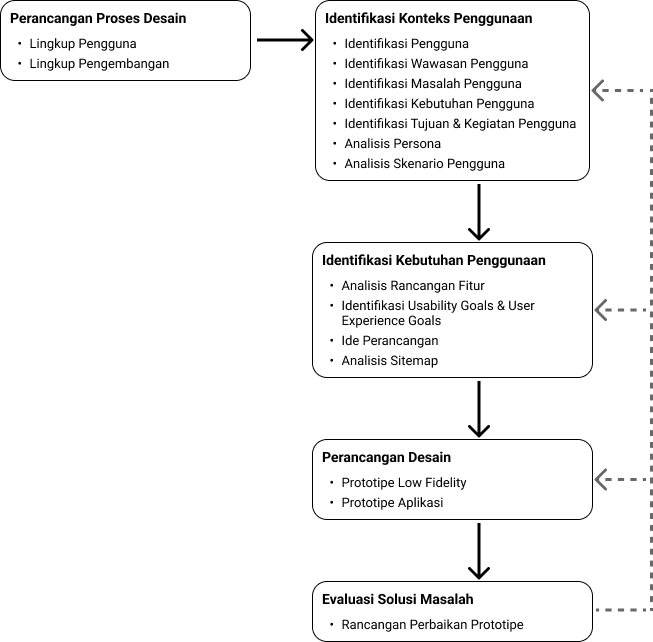
\includegraphics[width=0.8\textwidth]{chapter-3-alur-penelitian.png}
%   \caption{Alur Kerja Penelitian}
%   \label{fig:diagram_alur_kerja}
% \end{figure}

% \subsection{Perancangan Proses Desain}
% Ruang lingkup yang ditentukan pada penelitian ini adalah sebagai berikut

% \begin{enumerate}
%   \item Lingkup Pengguna
%   \subitem Target pengguna dari penelitian ini adalah masyarakat Indonesia yang pernah menggunakan atau memiliki ketertarikan terhadap aplikasi pencegah distraksi. Rentang usia dari target pengguna tidak dibatasi, namun difokuskan kepada golongan \textit{millenials} dengan rentang usia 18-30 tahun.
%   \item Lingkup Pengembangan
%   \subitem Desain interaksi aplikasi pencegah distraksi yang dibuat memiliki bentuk \textit{mobile interface} dengan mewujudkan sebuah prototipe aplikasi dalam \textit{platform Android}. Aplikasi Digital Wellbeing milik Google ditetapkan menjadi garis dasar pengembangan prototipe aplikasi tersebut.
% \end{enumerate}


% \subsection{Identifikasi Konteks Penggunaan}

% Pada tahap ini dilakukan analisis hasil riset penggunaanalisis terhadap hasil riset yang


% \subsection{Identifikasi Kebutuhan Pengguna}


% \subsection{Perancangan Desain}


% \subsection{Evaluasi Solusi Masalah}



% % Ketiga solusi yang telah diuraikan pada subbab \ref{sec:analisis_solusi} akan diimplementasikan dalam prototipe aplikasi, beserta fitur-fitur lain pada Digital Wellbeing yang akan mendukung solusi tersebut. Prototipe aplikasi ini akan diimpementasikan pada \textit{platform} Android. Secara garis besar, proses perancangan prototipe aplikasi akan menggunakan pendekatan \textit{user-centered design} (UCD).

% Seperti yang telah disebutkan pada subbab \ref{sec:metodologi}, metodologi yang digunakan dalam pengerjaan Tugas Akhir ini akan menggunakan pendekatan UCD. Dengan maksud mengikuti prosesnya, maka langkah selanjutnya yang akan dilakukan adalah mengumpulkan data. Pengumpulan data akan dilakukan dengan menyebarkan form secara online serta melakukan wawancara dengan responden yang bersedia untuk bekerja sama lebih lanjut. Proses ini akan dilaksanakan pada periode pengerjaan Tugas Akhir 2. Pengumpulan data ini bertujuan untuk melakukan validasi terhadap permasalahan yang sudah dianalisis, dan juga tidak menutup kemungkinan untuk menemukan permasalahan desain interaksi lain dari masukan pengguna.

% Setelah melakukan pengumpulan data, akan dilakukan analisis terhadap masukan yang didapat untuk mejadi kebutuhan perangkat lunak. Hasil analisis juga akan memvalidasi analisis masalah dan solusi yang didapat dari observasi penulis pada subbab \ref{sec:analisis_masalah} dan \ref{sec:analisis_solusi}.

% Kebutuhan perangkat lunak yang telah disusun akan diimplementasi dalam bentuk prototipe \textit{low-fidelity} terlebih dahulu. Setelah dilakukan evaluasi, maka implementasi akan dilanjutkan dalam bentuk prototipe \textit{high-fidelity}. Setelah menjalani evaluasi, maka perancangan prototipe aplikasi akan dikerjakan. Prototipe aplikasi diharapkan akan menghasilkan data dengan kualitas yang lebih tinggi pada saat evaluasi dibandingkan saat menggunakan prototipe \textit{low-fidelity} atau \textit{high-fidelity}. Hasil evaluasi juga akan menentukan apakah aplikasi akan menjalani proses iterasi atau diimplementasi lebih lanjut.

% \blindtext